\documentclass{beamer}
\usepackage[utf8x]{inputenc}
\usepackage{ucs}
\usepackage{amsmath,tabularx}
\usetheme{CambridgeUS}
% \usecolortheme{crane}
% \usefonttheme{structurebold}
\newcolumntype{C}{>{\centering\arraybackslash}X}
\linespread{1.5}

\usepackage{subfigure}
\title[Of Mice and TCR]{\sc{Difference in Immunity Systems Of Mice From Two TCR Groups}}
\author[SD, WH, YL, SM]{Somak Dutta, Wooseok Ha, Yuefeng Liang, and Shailee Mehta\\Clients: Benjamin McDonald \& Albert Bendelac, Pathology.}

\institute[UChicago]{University of Chicago}
\date[22.04.2014]{April 22, 2014}

\usepackage{amsmath,supertabular,tabularx,graphicx,amssymb,amsfonts}
\usepackage{natbib,rotating}
\usepackage{default}
\newcolumntype{Z}{>{\centering\arraybackslash}X}%
% \titlegraphic{\includegraphics[width=20mm]{USTL}}
% \date{2005}




\renewcommand{\t}{\ensuremath{\theta}}
\renewcommand{\a}{\ensuremath{\alpha}}
\renewcommand{\b}{\ensuremath{\beta}}
\newcommand{\g}{\ensuremath{\gamma}}
\newcommand{\E}{\mathsf{E}}
\renewcommand{\d}{\ensuremath{\delta}}
\newcommand{\e}{\ensuremath{\epsilon}}
\newcommand{\s}{\sigma}
% \renewcommand{\S}{\Sigma}
\newcommand{\from}{\ensuremath{\leftarrow}}
\newcommand{\bm}{\mathbf}
\renewcommand{\l}{\lambda}
\newcommand{\dint}{\int\displaylimits}
\newcommand{\bx}{\mathbf x}
\newcommand{\by}{\mathbf y}
\newcommand{\be}{\pmb\e}
\renewcommand{\k}{\kappa}
\newcommand{\m}{\mu}
\newcommand{\A}{\ensuremath{\mathcal{A}}}
\newcommand{\B}{\ensuremath{\mathcal{B}}}
\newcommand{\sT}{\mathrm{T}}
\newcommand{\diag}{\mathrm{diag}}
\newcommand{\Tr}{\mathrm{Tr}}
\newcommand{\cov}{\mathbb{C}\mathrm{ov}~}
\newcommand{\var}{\mathbb{V}\mathrm{ar}~}

\begin{document}
\begin{frame}<handout:0>
  \titlepage
\end{frame}

%%%%%%%%%%%%%%%%%%%

\begin{frame}
 \frametitle{Raised hands?}
 \begin{tiny}
 The client is interested in studying the development of a population of immune system cells (T cells) located in three glands: spleen, thymus and the intraepithelial lymphocyte (IEL). To this end, the client has bred a total of 39 mice broadly categorized into two groups (C \& U) by their TCR, which in turn have 5 and 3 subcategories respectively based on the TCR subtypes. For each mice and each gland, the client obtained the ratio of two types of cell counts. The cell-count ratio is the variable that is used to test for any significant differences between the TCR development in the two categories of mice. \alert{ \bf THIS SENTENCE IS AN EXPERIMENT TO SEE IF PEOPLE ACTUALLY READ THE WHOLE ABSTRACT; PLEASE RESPOND BY RAISING A HAND DURING THE PRESENTATION}.  Our main contribution is to account for the within subtype correlation and thus making more sensible inference out of the data. We will also discuss issues like imbalance in the design created by the cost of the experiment.
  \end{tiny}
\end{frame}


\begin{frame}
 \frametitle{What are we talking about?}
%  \begin{block}
 \begin{itemize}
  \item T--cells are a type of lymphocyte that play a central role in cell-mediated immunity. \alert{T cells are GOOD CELLS}.
  \item A T cell receptor or \alert {TCR} is a molecule that is found on T--cells.
  \item TCR recognizes antigens.
  \item Thus TCR is linked with the immunity system of a mammal (contrary to the T--virus which create zombies).
  \end{itemize}
%    \end{block}
\end{frame}

\begin{frame}
\frametitle{Types of T--cells}
 \begin{center}
  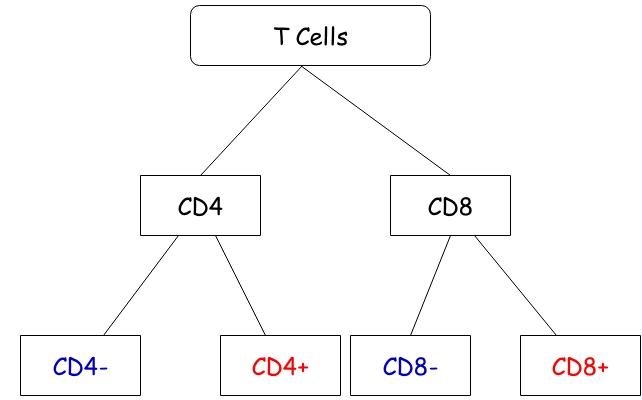
\includegraphics[width=0.8\textwidth]{TCELLS}
 \end{center}
\end{frame}


\begin{frame}
 \frametitle{Two types of TCR: C and U}
 \framebox{Q: Type {\alert C} and \alert{U} -- which one increases immunity?}
 
 \begin{itemize}
  \item Response: $\log\dfrac{\# \textsf{T CELL \bf +}}{\#\textsf{T CELL \bf --}}$.
  \item Cells from three glands: \alert{Thymus}, \alert{Spleen} and intraepithelial lymphocyte (\alert{IEL})
  \item Each TCR has subtypes:
   \begin{enumerate}
    \item TCR \alert{C} has \alert{5} subtypes: C1,\ldots,C5.
    \item TCR \alert{U} has \alert{4} subtypes: U1,\ldots,U4.
   \end{enumerate}

 \end{itemize}
\end{frame}

\begin{frame}
\frametitle{Plot of the data for thymus.}
Two sample t-statistic: 7.61 on 40 d.f., p-value $\approx 0$.
\begin{figure}
\centering 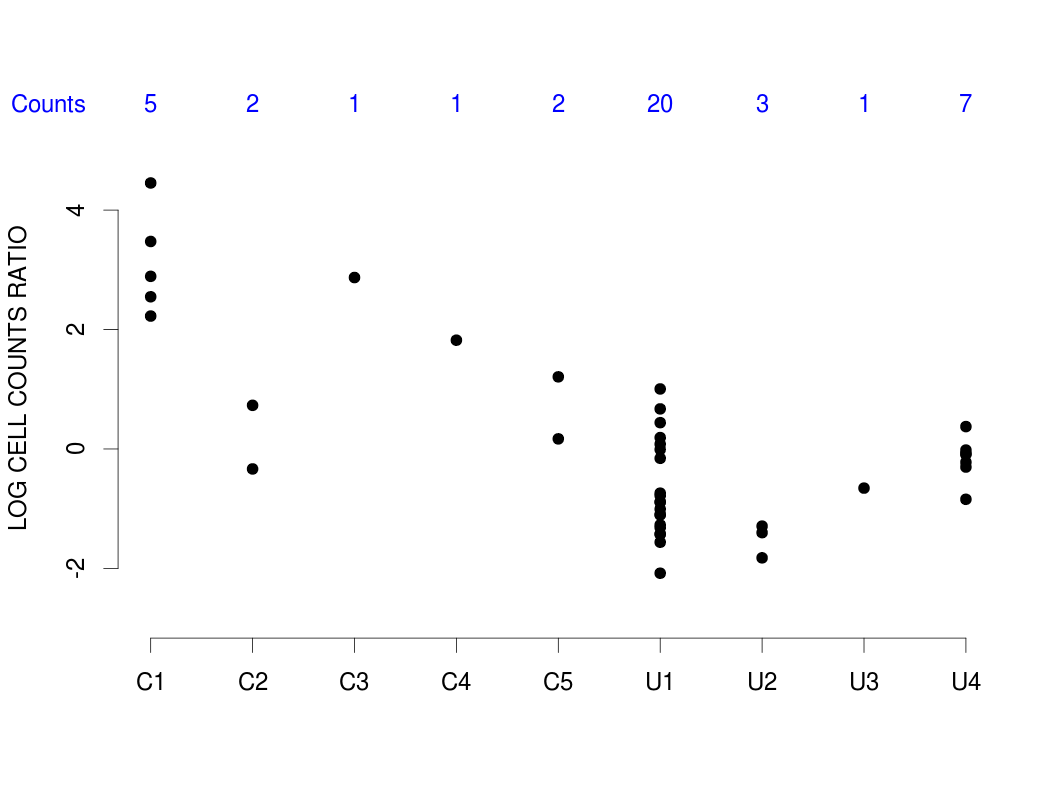
\includegraphics[width=0.7\textwidth]{plot_thymus}
\end{figure}
\end{frame}

\begin{frame}
\frametitle{Plot of the data for spleen.}
Two sample t-statistic = 5.98 on \alert{11.32} d.f., p-value = 0.0001.
\begin{center}
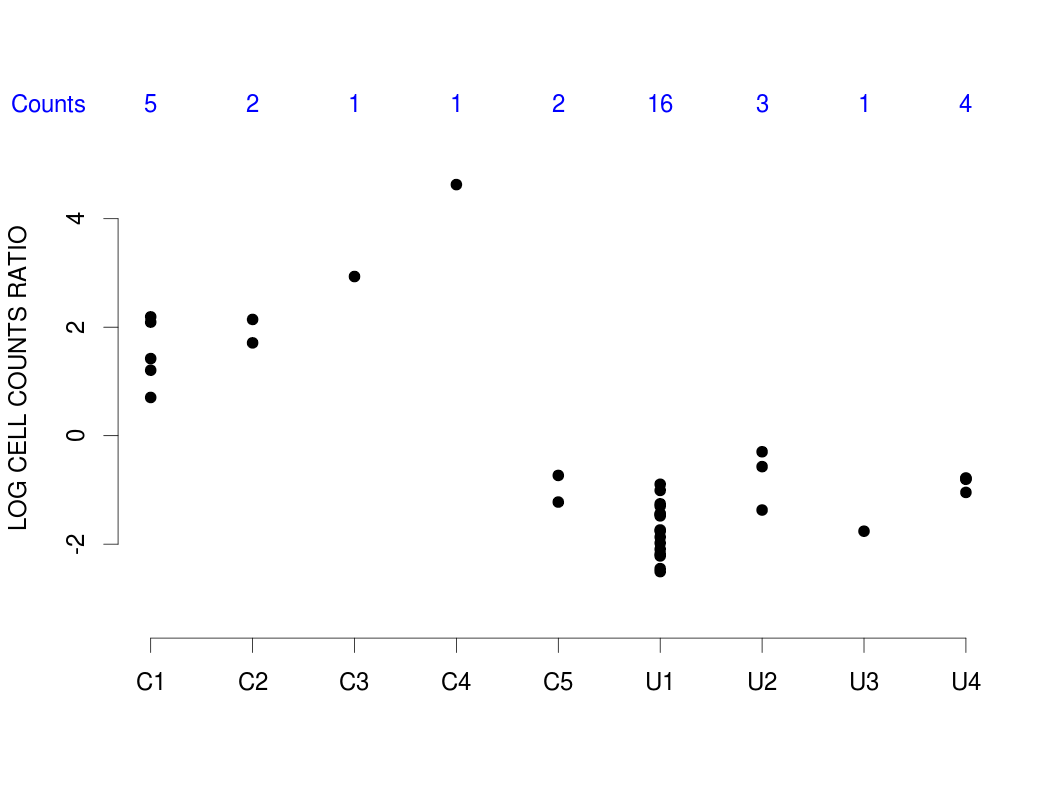
\includegraphics[width=0.8\textwidth]{plot_spleen}
\end{center}
\end{frame}

\begin{frame}
\frametitle{Plot of the data for IEL.}
Two sample t-statistic = 4.39 on  \alert{12.2} d.f., p-value = 0.0008.
\begin{center}
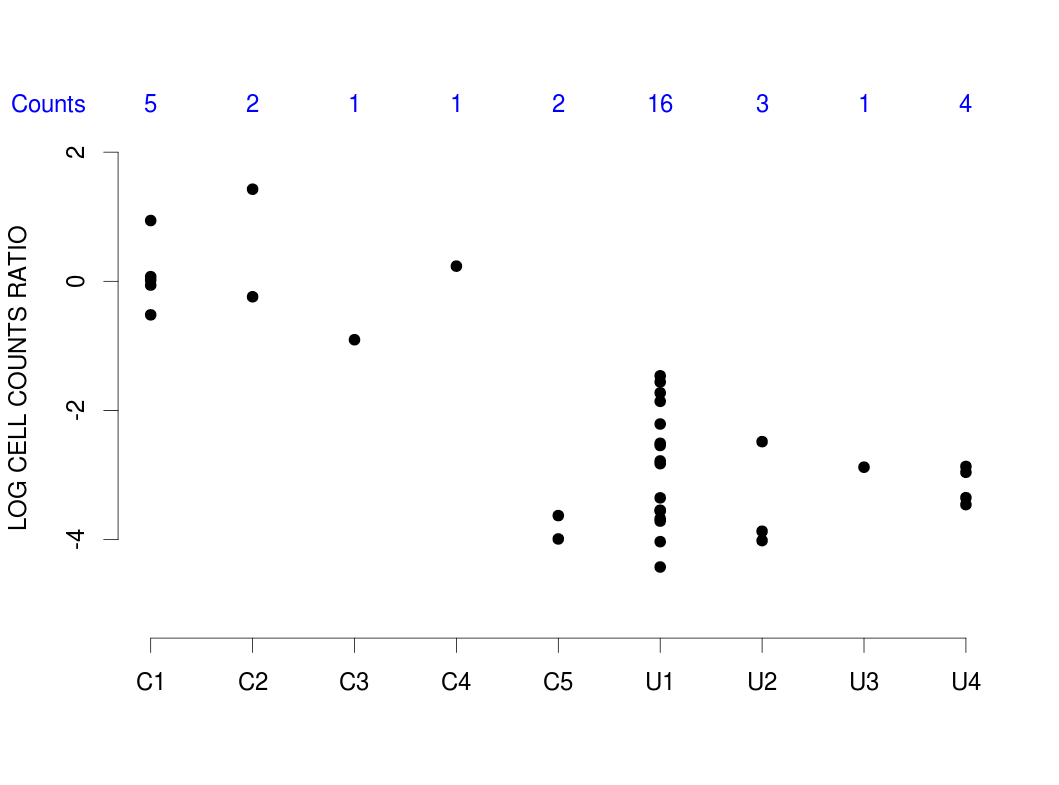
\includegraphics[width=0.8\textwidth]{plot_iel}
\end{center}
\end{frame}

\begin{frame}
\frametitle{MODEL FOR EACH GLAND }
Gaussian model for the log-response:
For $i$th and $j$th mice, $i\neq j$
\begin{eqnarray*}
\log \textsf{ratio} & \sim & \mathcal{N}(\pmb\mu,\Sigma) \\
\mu_i & = & \alpha + \beta_{type(i)} \qquad type(i) \in \{C,U\} \\
\Sigma_{ii} & = & \sigma^2 + \sigma_{st}^2,	\qquad marginal~variance.\\
\Sigma_{i,j} & = & \begin{cases}
\sigma_{st}^2, & \textsf{if } i\neq j \textsf{ have same TCR subtype.}\\
0 & \textsf{otherwise} \\
                   \end{cases}
\end{eqnarray*}

\begin{center}
\framebox{\alert{Person of interest: $\beta_C - \beta_U$}} 
\end{center}
\end{frame}

\begin{frame}
\frametitle{Estimates using REML: $\beta_C-\beta_U$}
\begin{eqnarray*}
\mu_i & = & \alpha + \beta_{type(i)} \qquad type(i) \in \{C,U\} \\
\end{eqnarray*}

\begin{center}
\begin{tabular}{|c| c | c | c |  c|}\hline
Gland & Estimate & s.e. & t-ratio & p-value \\ \hline
Thymus & 2.46 & 0.71 & 3.49 &  0.010 \\ \hline
Spleen & 3.24 & 1.05 & 3.08 &  0.018 \\ \hline
IEL &  2.33 & 0.91 & 2.55 &   0.038 \\  \hline
\end{tabular}
\end{center}
\end{frame}



\begin{frame}
\frametitle{Estimates using REML: Variance components}
\begin{eqnarray*}
\Sigma_{ii} & = & \sigma^2 + \sigma_{st}^2,	\qquad marginal~variance.\\
\Sigma_{i,j} & = & \begin{cases}
\sigma_{st}^2, & \textsf{if } i\neq j \textsf{ have same TCR subtype.}\\
0 & \textsf{otherwise} \\
                   \end{cases}
\end{eqnarray*}

\begin{center}
\begin{tabular}{|c| c  c | c   c|}\hline
Gland & Parameter & Estimate (s.e.) & Parameter & Estimate (s.e.) \\ \hline 
Thymus & $\sigma^2$ &  0.551 (0.135)& $\sigma_{st}^2$ & 0.871      (0.604) \\ \hline 
Spleen & $\sigma^2$ &  0.234 (0.065)& $\sigma_{st}^2$ &2.334      (1.313) \\ \hline
IEL & $\sigma^2$ &  0.663 (0.184) & $\sigma_{st}^2$ & 1.536 (1.000) \\ \hline
\end{tabular}
\end{center}
\end{frame}


\begin{frame}
\frametitle{Comments}
\begin{enumerate}
 \item Imbalance in design caused by cost of breeding mice of certain subtypes.
 \item The mixed linear models fit the data better (higher log-likelihood values).
 \item Client happy with higher (but still significant) p-values.
\end{enumerate}
\end{frame}

\usebackgroundtemplate{
\includegraphics[width=\paperwidth]{thanks}}%
\begin{frame}
\frametitle{Thank You}

\end{frame}

\end{document}

